\documentclass[12pt,a4paper]{book}

\usepackage[T1]{fontenc}
\usepackage[utf8]{inputenc}
\usepackage{lmodern}
\usepackage[a4paper, top=2.5cm, bottom=2.5cm, left=3cm, right=2.5cm]{geometry}
\usepackage{graphicx}
\usepackage{xcolor}
\usepackage{titlesec}
\usepackage{tocloft}
\usepackage{fancyhdr}
\usepackage{hyperref}
\usepackage{enumitem}
\usepackage{booktabs}
\usepackage{array}
\usepackage{amssymb}
\usepackage{tabularx}
\usepackage{fontawesome5}
% Fallback definitions for FontAwesome icons used in AmarVote TeX guides.
% If the icon macro is already defined by fontawesome5, \providecommand will leave it untouched.
\providecommand{\faCalculator}[1][]{ }
\providecommand{\faCalendarAlt}[1][]{ }
\providecommand{\faChartBar}[1][]{ }
\providecommand{\faCheck}[1][]{ }
\providecommand{\faCheckDouble}[1][]{ }
\providecommand{\faChevronRight}[1][]{ }
\providecommand{\faCircle}[1][]{ }
\providecommand{\faCog}[1][]{ }
\providecommand{\faCopy}[1][]{ }
\providecommand{\faEnvelope}[1][]{ }
\providecommand{\faExclamationCircle}[1][]{ }
\providecommand{\faExclamationTriangle}[1][]{ }
\providecommand{\faFlask}[1][]{ }
\providecommand{\faiBell}[1][]{ }
\providecommand{\faInfoCircle}[1][]{ }
\providecommand{\faKey}[1][]{ }
\providecommand{\faLayerGroup}[1][]{ }
\providecommand{\faLightbulb}[1][]{ }
\providecommand{\faLock}[1][]{ }
\providecommand{\faLockOpen}[1][]{ }
\providecommand{\faPlusCircle}[1][]{ }
\providecommand{\faSearch}[1][]{ }
\providecommand{\faShieldAlt}[1][]{ }
\providecommand{\faTimes}[1][]{ }
\providecommand{\faTimesCircle}[1][]{ }
\providecommand{\faUser}[1][]{ }
\providecommand{\faUserPlus}[1][]{ }
\providecommand{\faUserShield}[1][]{ }
\providecommand{\faVoteYea}[1][]{ }

\usepackage{tikz}
\usetikzlibrary{shapes.geometric,arrows.meta,positioning,calc}
\usepackage{microtype}
\usepackage{setspace}
\usepackage{parskip}
\usepackage{float}
\usepackage{colortbl}
\usepackage{longtable}
\usepackage{tcolorbox}
\tcbuselibrary{skins,breakable}

% ─── Colours ─────────────────────────────────────────────────────────────────
\definecolor{guardgreen}{HTML}{145A32}
\definecolor{guardaccent}{HTML}{1E8449}
\definecolor{coverbg}{HTML}{071A0E}
\definecolor{lightgray}{HTML}{F5F7FA}
\definecolor{warningyellow}{HTML}{FFF3CD}
\definecolor{warningborder}{HTML}{FBBF24}
\definecolor{successgreen}{HTML}{D1FAE5}
\definecolor{successborder}{HTML}{10B981}
\definecolor{infoblue}{HTML}{DBEAFE}
\definecolor{infoborder}{HTML}{3B82F6}
\definecolor{dangered}{HTML}{FEE2E2}
\definecolor{dangerborder}{HTML}{EF4444}
\definecolor{sectiongray}{HTML}{6B7280}

\hypersetup{
  colorlinks=true,linkcolor=guardgreen,
  urlcolor=guardaccent,citecolor=guardaccent,
  pdftitle={AmarVote --- Guardian Guide},
}

\tcbset{
  notebox/.style={enhanced,breakable,colback=infoblue,colframe=infoborder,
    fonttitle=\bfseries\color{guardgreen},title={\faInfoCircle\quad Note},
    left=6pt,right=6pt,top=4pt,bottom=4pt,arc=4pt},
  warnbox/.style={enhanced,breakable,colback=warningyellow,colframe=warningborder,
    fonttitle=\bfseries\color{orange!80!black},title={\faExclamationTriangle\quad Important},
    left=6pt,right=6pt,top=4pt,bottom=4pt,arc=4pt},
  tipbox/.style={enhanced,breakable,colback=successgreen,colframe=successborder,
    fonttitle=\bfseries\color{green!50!black},title={\faLightbulb\quad Tip},
    left=6pt,right=6pt,top=4pt,bottom=4pt,arc=4pt},
  dangerbox/.style={enhanced,breakable,colback=dangered,colframe=dangerborder,
    fonttitle=\bfseries\color{red!70!black},title={\faTimesCircle\quad Critical},
    left=6pt,right=6pt,top=4pt,bottom=4pt,arc=4pt},
  phasebox/.style={enhanced,breakable,colback=successgreen!50!white,colframe=guardgreen,
    fonttitle=\bfseries\color{white},
    attach boxed title to top left={xshift=10pt,yshift=-\tcboxedtitleheight/2},
    boxed title style={colback=guardgreen,arc=3pt},
    left=6pt,right=6pt,top=14pt,bottom=4pt,arc=4pt},
  cryptobox/.style={enhanced,breakable,colback=lightgray,colframe=guardaccent,
    fonttitle=\bfseries\color{guardgreen},title={\faLock\quad Cryptographic Concept},
    left=8pt,right=8pt,top=6pt,bottom=6pt,arc=6pt},
}

\titleformat{\chapter}[display]
  {\normalfont\huge\bfseries\color{guardgreen}}
  {\chaptertitlename\ \thechapter}{12pt}{\Huge}
\titlespacing{\chapter}{0pt}{-10pt}{20pt}
\titleformat{\section}{\normalfont\Large\bfseries\color{guardgreen}}{\thesection}{1em}{}
\titleformat{\subsection}{\normalfont\large\bfseries\color{guardaccent}}{\thesubsection}{1em}{}
\titleformat{\subsubsection}{\normalfont\normalsize\bfseries\color{sectiongray}}{\thesubsubsection}{1em}{}

\pagestyle{fancy}
\fancyhf{}
\fancyhead[LE,RO]{\small\thepage}
\fancyhead[LO]{\small\nouppercase{\rightmark}}
\fancyhead[RE]{\small\nouppercase{\leftmark}}
\fancyfoot[C]{\small\color{sectiongray}AmarVote --- Guardian Guide}
\renewcommand{\headrulewidth}{0.4pt}

\setlist[itemize,1]{label=\textcolor{guardaccent}{\faChevronRight},leftmargin=1.5em}
\setlist[itemize,2]{label=\textcolor{sectiongray}{\faCircle[regular]},leftmargin=2em}
\setlist[enumerate,1]{label=\textcolor{guardgreen}{\textbf{\arabic*.}},leftmargin=2em}

\newcommand{\uibutton}[1]{\colorbox{guardgreen}{\textcolor{white}{\small\textbf{#1}}}}
\newcommand{\uifield}[1]{\texttt{\color{guardaccent}#1}}
\newcommand{\uimenu}[1]{\textbf{\color{guardgreen}#1}}

\setstretch{1.15}

\begin{document}

% ─── COVER ───────────────────────────────────────────────────────────────────
\begin{titlepage}
\pagecolor{coverbg}
\color{white}
\centering
\vspace*{1.5cm}

{\fontsize{55}{60}\selectfont\bfseries AmarVote}

\vspace{0.4cm}
{\large\color{guardaccent} Secure Cryptographic Voting Platform}

\vspace{1.5cm}
\hrule width 13cm height 0.5pt
\vspace{0.5cm}
{\LARGE\bfseries \faShieldAlt\quad Guardian Guide}
\vspace{0.5cm}
\hrule width 13cm height 0.5pt

\vspace{2cm}

\begin{tcolorbox}[
  enhanced,width=11cm,
  colback=guardgreen!30!black,colframe=guardaccent,
  arc=6pt,boxrule=1.5pt,left=14pt,right=14pt,top=10pt,bottom=10pt
]
\centering\color{white}
\textbf{Your responsibilities as a Guardian:}\\[8pt]
\textcolor{guardaccent}{\faUserShield} \, Account Registration \& Login\\[4pt]
\textcolor{guardaccent}{\faKey} \, Phase 1: Key Pair Generation\\[4pt]
\textcolor{guardaccent}{\faCopy} \, Phase 2: Backup Share Generation\\[4pt]
\textcolor{guardaccent}{\faLockOpen} \, Partial \& Compensated Decryption\\[4pt]
\textcolor{guardaccent}{\faLayerGroup} \, Combining Decryption Shares
\end{tcolorbox}

\vfill
{\small\color{sectiongray}
  \faExclamationCircle\quad This guide contains critical security instructions.\\
  Read every warning box carefully.
}
\vspace{1cm}
{\small Version 1.0 \quad|\quad \today}
\end{titlepage}
\nopagecolor\color{black}

\frontmatter
\tableofcontents

\chapter*{Your Role as a Guardian}
\addcontentsline{toc}{chapter}{Your Role as a Guardian}

You have been assigned as a \textbf{Guardian} for an AmarVote election. This is a position of significant trust and responsibility.

\textbf{What does a Guardian do?}

In AmarVote, no single person can decrypt the election results alone. Instead, the decryption key is mathematically distributed among all guardians using a technique called \emph{threshold cryptography}. To decrypt the tally and reveal the results, a minimum number of guardians (the \emph{quorum}) must cooperate.

\textbf{Why is this important?}

This means:
\begin{itemize}
  \item Even the election administrator cannot manipulate or see individual votes.
  \item Even if one guardian is malicious, they cannot singlehandedly decrypt the tally.
  \item Even if some guardians are unavailable, the election can still be tallied (if enough guardians cooperate to meet the quorum).
\end{itemize}

\begin{tcolorbox}[warnbox]
\textbf{Your two most critical responsibilities:}
\begin{enumerate}
  \item \textbf{Securely store} your encrypted private key file (downloaded in Phase 1).
  \item \textbf{Remember or safely store} your Guardian Password.
\end{enumerate}
If you lose either of these, you may prevent the election results from ever being published.
\end{tcolorbox}

\mainmatter

% ════════════════════════════════════════════════════════════════════════════
\chapter{Account Setup: Registration \& Login}
\label{ch:guard-account}

Before performing any guardian duties, you need a registered AmarVote account.

\section{Prerequisites}

Your email address must be on the \textbf{Authorised User List}. The election administrator or platform Owner will have added you. If you are unsure, contact the election administrator.

\section{Registering Your Account}

\begin{enumerate}
  \item Open your browser and navigate to the AmarVote URL.
  \item Click \uibutton{Register} or go to \texttt{/register}.
  \item Enter your authorised email address in the \uifield{Email Address} field.
  \item Click \uibutton{Send Verification Code}.
  \item Check your email inbox for a 6-digit One-Time Password (OTP) from AmarVote. Check your spam folder if you don't see it within 2 minutes.
  \item Enter the OTP in the \uifield{Verification Code} field.
  \item Click \uibutton{Verify Email}.
  \item Create a strong password (12+ characters, mixed case, numbers, symbols).
  \item Confirm the password in the \uifield{Confirm Password} field.
  \item Click \uibutton{Create Account}.
\end{enumerate}

\begin{tcolorbox}[dangerbox]
As a Guardian, your account credentials protect the election's cryptographic infrastructure. Use a strong, unique password and store it in a password manager. Do not reuse passwords from other services.
\end{tcolorbox}

\section{Enabling Two-Factor Authentication}

2FA is strongly recommended for all guardian accounts.

\begin{enumerate}
  \item After logging in, click your avatar and select \uimenu{Profile Settings}.
  \item Under \uimenu{Security}, click \uibutton{Enable Two-Factor Authentication}.
  \item Scan the QR code with Google Authenticator or any TOTP app.
  \item Enter the current 6-digit code from the app and click \uibutton{Activate}.
  \item \textbf{Save the displayed recovery codes} in a secure location.
\end{enumerate}

\section{Logging In}

\begin{enumerate}
  \item Navigate to the AmarVote URL and click \uibutton{Login}.
  \item Enter your \uifield{Email Address} and \uifield{Password}.
  \item If 2FA is enabled: enter the 6-digit TOTP code from your authenticator app.
  \item Click \uibutton{Sign In}.
\end{enumerate}

% ════════════════════════════════════════════════════════════════════════════
\chapter{Understanding the Key Ceremony}
\label{ch:guard-ceremony-overview}

Before diving into the steps, it is worth understanding \emph{what} you are doing and \emph{why}. This chapter gives a conceptual overview.

\section{The Three-Phase Ceremony}

\begin{center}
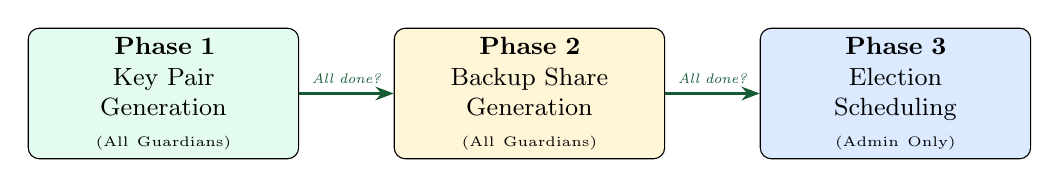
\begin{tikzpicture}[node distance=1.2cm,
  block/.style={draw,fill=lightgray,rounded corners,text width=3.2cm,align=center,minimum height=1.4cm,font=\small},
  arrow/.style={-Stealth,thick,color=guardgreen}
]
  \node[block,fill=successgreen!60!white] (P1) {\textbf{Phase 1}\\Key Pair\\Generation\\{\tiny(All Guardians)}};
  \node[block,fill=warningyellow!80!white,right=of P1] (P2) {\textbf{Phase 2}\\Backup Share\\Generation\\{\tiny(All Guardians)}};
  \node[block,fill=infoblue,right=of P2] (P3) {\textbf{Phase 3}\\Election\\Scheduling\\{\tiny(Admin Only)}};
  \draw[arrow] (P1) -- (P2) node[midway,above,font=\tiny\itshape]{All done?};
  \draw[arrow] (P2) -- (P3) node[midway,above,font=\tiny\itshape]{All done?};
\end{tikzpicture}
\end{center}

\begin{tcolorbox}[cryptobox]
\textbf{Asymmetric cryptography basics:}
\begin{itemize}
  \item A \textbf{key pair} consists of a \textbf{public key} and a \textbf{private key}.
  \item Anything encrypted with a public key can \emph{only} be decrypted with the matching private key.
  \item In AmarVote, ballots are encrypted with a combined election public key. Decryption requires guardian private keys (above the quorum threshold).
\end{itemize}
\end{tcolorbox}

\section{What Happens to Your Key}

\begin{itemize}
  \item \textbf{Your public key} is stored in the AmarVote database and used in ballot encryption.
  \item \textbf{Your private key} is \emph{never} stored on the server. It is encrypted with your password using AES-256 and stored only on your device.
  \item \textbf{Backup shares} of your private key are split into $(n-1)$ fragments (where $n$ is the total number of guardians) and each fragment is encrypted with a different guardian's public key. These encrypted fragments are stored in the database.
\end{itemize}

\begin{tcolorbox}[notebox]
\textbf{Why backup shares matter:} If you cannot participate in decryption, the other guardians can use your backup shares (which only they can decrypt) to reconstruct your key contribution. This is how the system tolerates absent guardians while maintaining the quorum requirement.
\end{tcolorbox}

% ════════════════════════════════════════════════════════════════════════════
\chapter{Phase 1: Key Pair Generation}
\label{ch:guard-phase1}

\begin{tcolorbox}[phasebox,title={Phase 1: Key Pair Generation}]
\textbf{When:} Immediately after election creation.\\
\textbf{Who:} All guardians (each independently).\\
\textbf{Blocking:} Phase 2 cannot begin until \emph{all} guardians complete Phase 1.\\
\textbf{Output:} One public key (uploaded to server) + one encrypted private key file (downloaded to your device).
\end{tcolorbox}

\section{Finding Your Election}

\begin{enumerate}
  \item Log in to AmarVote.
  \item You may see a notification in the \faiBell\ Notifications area indicating you have a guardian assignment. Click it to go directly to the election, \emph{or}:
  \item Navigate to \uimenu{All Elections} in the sidebar.
  \item Find the election for which you are a guardian and click on it to open the election page.
\end{enumerate}

\section{Accessing the Guardian Tab}

\begin{enumerate}
  \item On the election page, look for the tab bar near the top.
  \item Click the \uimenu{Guardian} tab.
  \item You will see the Key Ceremony status panel. Phase 1 should be marked as \textbf{Active}.
\end{enumerate}

\section{Generating Your Key Pair}

\begin{enumerate}
  \item In the Phase 1 panel, click \uibutton{Generate Key Pair}.
  \item The system will cryptographically generate your unique asymmetric key pair for this election. This happens entirely in your browser --- the private key never leaves your device unencrypted.
  \item A password prompt will appear with two options:
\end{enumerate}

\subsection{Setting Your Guardian Password}

\begin{center}
\begin{tabularx}{0.9\textwidth}{>{\bfseries}l X}
\toprule
\rowcolor{guardgreen}\color{white}Option & \color{white}What It Does \\
\midrule
\rowcolor{lightgray}Generate Secure Password & The system generates a cryptographically random, high-entropy password. Recommended. \\
Enter Your Own Password & You type a password of your choice. Must be strong (see requirements below). \\
\bottomrule
\end{tabularx}
\end{center}

\begin{tcolorbox}[dangerbox]
\textbf{This password is irreplaceable.} There is no ``forgot password'' for the guardian password. If you forget it, your private key file is permanently inaccessible, and you will be unable to participate in decryption.
\end{tcolorbox}

\begin{tcolorbox}[tipbox]
Use the \uibutton{Generate Secure Password} button. Then immediately copy the generated password and save it in your password manager with a label like \texttt{AmarVote Guardian Password - [Election Name]}.
\end{tcolorbox}

\section{Submitting and Downloading}

\begin{enumerate}
  \item Once you have set and recorded your password, click \uibutton{Submit Key Pair \& Download}.
  \item Two things happen simultaneously:
  \begin{enumerate}
    \item Your \textbf{public key} is transmitted to the AmarVote server and stored in the database.
    \item An \textbf{encrypted private key file} (e.g., \texttt{guardian\_key\_[yourname]\_[election\_id].enc}) is automatically downloaded to your browser's default downloads folder.
  \end{enumerate}
  \item A green success message will appear: ``Phase 1 Complete''.
\end{enumerate}

\section{Immediately After Downloading}

\begin{enumerate}
  \item Move the downloaded \texttt{.enc} file to a \textbf{secure, backed-up location}:
  \begin{itemize}
    \item An encrypted USB drive (stored securely offline)
    \item An encrypted cloud storage folder (e.g., encrypted with VeraCrypt before upload)
    \item Your system's encrypted home directory (ensure full-disk encryption is enabled)
  \end{itemize}
  \item Do \textbf{not} leave it in your Downloads folder indefinitely.
  \item Verify your password is saved in your password manager.
\end{enumerate}

\begin{tcolorbox}[warnbox]
\textbf{Do not share the private key file or your guardian password with anyone} --- including the election administrator. Sharing these would compromise the security guarantee of the election.
\end{tcolorbox}

% ════════════════════════════════════════════════════════════════════════════
\chapter{Phase 2: Backup Share Generation}
\label{ch:guard-phase2}

\begin{tcolorbox}[phasebox,title={Phase 2: Backup Share Generation}]
\textbf{When:} After all guardians complete Phase 1.\\
\textbf{Who:} All guardians (each independently).\\
\textbf{Blocking:} Phase 3 (election scheduling) cannot begin until all guardians complete Phase 2.\\
\textbf{Output:} Encrypted backup shares stored in the server database.
\end{tcolorbox}

\section{What Backup Shares Are}

\begin{tcolorbox}[cryptobox]
\textbf{Shamir's Secret Sharing (simplified):} Your private key is mathematically split into $n-1$ fragments (where $n$ is the total number of guardians). Each fragment is encrypted using the public key of a different guardian. Only that guardian can decrypt their fragment. If quorum-many guardians each provide their fragment, the original private key can be reconstructed --- but no single fragment reveals anything on its own.
\end{tcolorbox}

\textbf{Example with 5 guardians, quorum = 3:}
\begin{itemize}
  \item Guardian G1 generates 4 backup fragments (for G2, G3, G4, G5).
  \item The fragment for G2 is encrypted with G2's public key --- only G2 can open it.
  \item If G1 is missing during decryption, G2, G3, and G4 can each provide their fragment of G1's key. With 3 fragments (meeting quorum), G1's key is reconstructed.
\end{itemize}

\section{Generating Your Backup Shares}

\begin{enumerate}
  \item Navigate to the election page and open the \uimenu{Guardian} tab.
  \item Phase 2 should now show as \textbf{Active}.
  \item Click \uibutton{Upload Encrypted Key File} and select the \texttt{.enc} file you downloaded in Phase 1.
  \item Enter your \uifield{Guardian Password} in the provided field.
  \item Click \uibutton{Generate Backup Shares}.
  \item The browser will:
  \begin{enumerate}
    \item Decrypt your private key in memory using your password (via AES-256).
    \item Generate $n-1$ backup fragments from your private key.
    \item Encrypt each fragment with the corresponding guardian's public key.
    \item Transmit all encrypted fragments to the server.
    \item Erase the decrypted private key from memory.
  \end{enumerate}
  \item A success message will appear: ``Phase 2 Complete''.
\end{enumerate}

\begin{tcolorbox}[notebox]
The decryption of your private key happens \emph{entirely within your browser}, in memory, for only the duration of this process. Your password and private key are \textbf{never sent to the server}. Only the encrypted backup shares (which are meaningless without the recipient's private key) are transmitted.
\end{tcolorbox}

\begin{tcolorbox}[warnbox]
If you close the browser or lose your internet connection during backup share generation, the process may fail. Return to the Guardian tab and repeat the step --- it is safe to retry.
\end{tcolorbox}

\section{After Completing Phase 2}

After you submit your backup shares:
\begin{itemize}
  \item You do not need to take any further action until the election closes.
  \item You may optionally vote in the election if you are also on the voter list.
  \item Keep your private key file and password safe --- you will need them again for decryption.
\end{itemize}

% ════════════════════════════════════════════════════════════════════════════
\chapter{Waiting Period: During the Election}
\label{ch:guard-during}

After Phase 2, the election administrator will schedule the election and voters will cast their ballots. During this period, your guardian responsibilities are paused.

\section{What to Do During This Period}

\begin{itemize}
  \item \textbf{Keep your credentials safe}: Your private key file and guardian password must remain accessible to you after the election closes.
  \item \textbf{Watch for notifications}: AmarVote will notify you when the election closes and the tally phase begins.
  \item \textbf{Participate as a voter}: If you are on the voter list, you may cast your own ballot just like any other voter.
\end{itemize}

\begin{tcolorbox}[warnbox]
If you change devices, transfer your encrypted private key file to the new device \emph{before} the decryption phase begins. Ensure your password manager is synced.
\end{tcolorbox}

% ════════════════════════════════════════════════════════════════════════════
\chapter{Post-Election: Partial Decryption}
\label{ch:guard-decrypt}

After the election closes and the tally is computed (initiated by the admin), each guardian must perform their partial decryption. This is the step where your private key is used to ``unlock'' your share of the tally.

\section{When to Begin}

\begin{itemize}
  \item You will receive a notification that the tally is complete and decryption can begin.
  \item Navigate to the election page and open the \uimenu{Guardian} tab.
  \item You will see the \textbf{Partial Decryption} panel is now active.
\end{itemize}

\section{Performing Partial Decryption}

\begin{enumerate}
  \item Click \uibutton{Upload Encrypted Key File}.
  \item Select the \texttt{.enc} file from your secure storage location.
  \item Enter your \uifield{Guardian Password} in the provided field.
  \item Click \uibutton{Submit Credentials \& Decrypt}.
\end{enumerate}

\subsection{What Happens During Decryption}

The browser performs the following operations:

\begin{enumerate}
  \item \textbf{Credential Verification}: Your password decrypts your private key in memory. If the password is incorrect, an error is shown immediately.
  \item \textbf{Partial Decryption}: Your private key is applied to each chunk of the encrypted tally. This produces a \emph{partial decryption} for your guardian share --- a mathematical result that, when combined with others, will reveal the total.
  \item \textbf{Compensated Decryption}: For each \emph{other} guardian's backup share of \emph{your} key (stored in the database), your private key decrypts those shares and computes \emph{compensated decryption values}. These substitutes allow the system to account for guardians who cannot participate, without revealing their private keys.
  \item \textbf{Submission}: All partial and compensated decryption data is submitted to the server.
  \item \textbf{Memory Cleanup}: Your decrypted private key is erased from browser memory.
\end{enumerate}

\begin{tcolorbox}[warnbox]
\textbf{Do not close the browser tab} during this process. Partial decryption involves significant computation and may take several minutes depending on the number of ballot chunks (each chunk contains approximately 200 ballots).
\end{tcolorbox}

\begin{tcolorbox}[notebox]
\textbf{Progress tracking:} A progress bar will display the current chunk being processed vs. the total number of chunks. For a 2000-ballot election with 200-ballot chunks, there would be 10 chunks to process.
\end{tcolorbox}

\section{After Partial Decryption is Complete}

\begin{enumerate}
  \item A success message will confirm your partial and compensated decryptions have been submitted.
  \item Your guardian contribution is complete.
  \item The election page will show updated progress: how many of the required quorum have now submitted their decryptions.
  \item Once the quorum is met, either you or the admin can click \uibutton{Combine Decryption Shares}.
\end{enumerate}

% ════════════════════════════════════════════════════════════════════════════
\chapter{Combining Decryption Shares}
\label{ch:guard-combine}

When at least \emph{quorum} guardians have completed their partial decryption, the final results can be produced.

\section{Who Can Combine}

Both the election administrator and any guardian can initiate the combination step.

\section{Steps to Combine}

\begin{enumerate}
  \item Navigate to the election page's \uimenu{Tally} or \uimenu{Guardian} tab.
  \item Check the decryption status table --- confirm that the required number of guardians (at least quorum) show as \textbf{Complete}.
  \item Click \uibutton{Combine Decryption Shares}.
  \item The server will:
  \begin{enumerate}
    \item Retrieve all submitted partial decryptions.
    \item For absent guardians (below quorum threshold), substitute with compensated decryptions.
    \item Mathematically combine all shares using the ElectionGuard protocol.
    \item Produce the final plaintext vote totals.
    \item Publish the results with full cryptographic proofs.
  \end{enumerate}
  \item The results page will load automatically when the combination is complete.
\end{enumerate}

\begin{tcolorbox}[warnbox]
\textbf{Verify before combining.} Once you click \uibutton{Combine Decryption Shares}, the results are final and published. Make sure the correct number of guardians have completed decryption before proceeding.
\end{tcolorbox}

% ════════════════════════════════════════════════════════════════════════════
\chapter{Verifying the Results}
\label{ch:guard-verify}

As a guardian, you have a special responsibility to review the published results and confirm that the cryptographic proofs are valid.

\section{Reviewing Published Results}

\begin{enumerate}
  \item After combination, navigate to the \uimenu{Results} tab of the election.
  \item Review the vote totals, percentage breakdown, and total ballot count.
  \item Compare these results with your own expectations (if you monitored the election).
\end{enumerate}

\section{Downloading the Audit Package}

\begin{enumerate}
  \item Navigate to the \uimenu{Verification} tab.
  \item Click \uibutton{Download Election Data}.
  \item The package contains all cryptographic artefacts except private keys.
  \item Optionally, verify the data using ElectionGuard's open-source verifier tools.
\end{enumerate}

\begin{tcolorbox}[tipbox]
As a guardian who understands the cryptographic process, you are well-positioned to independently verify the election using ElectionGuard's reference verifier. This is the gold standard of election auditability.
\end{tcolorbox}

% ════════════════════════════════════════════════════════════════════════════
\appendix

\chapter{Guardian Security Checklist}

Complete this checklist before, during, and after your guardian duties:

\vspace{0.3cm}
\textbf{Before Phase 1:}
\begin{itemize}
  \item[$\square$] Registered AmarVote account with authorised email
  \item[$\square$] Enabled 2FA with Google Authenticator
  \item[$\square$] Set up password manager to store guardian password
  \item[$\square$] Identified a secure storage location for the private key file
\end{itemize}

\vspace{0.3cm}
\textbf{After Phase 1:}
\begin{itemize}
  \item[$\square$] Guardian password saved in password manager
  \item[$\square$] Private key file (\texttt{.enc}) downloaded
  \item[$\square$] Private key file moved to secure storage (not Downloads folder)
  \item[$\square$] Private key file backed up in at least one additional secure location
\end{itemize}

\vspace{0.3cm}
\textbf{After Phase 2:}
\begin{itemize}
  \item[$\square$] Backup shares successfully generated and submitted
  \item[$\square$] Confirmed Phase 2 status shows ``Complete'' for your guardian entry
  \item[$\square$] Private key file and password still securely stored (do not delete them!)
\end{itemize}

\vspace{0.3cm}
\textbf{After Election Closes (Decryption Phase):}
\begin{itemize}
  \item[$\square$] Located private key file in secure storage
  \item[$\square$] Retrieved guardian password from password manager
  \item[$\square$] Completed partial and compensated decryption
  \item[$\square$] Confirmed decryption submission success message
  \item[$\square$] If quorum is met: clicked Combine or confirmed admin has done so
\end{itemize}

\chapter{Frequently Asked Questions for Guardians}

\section*{What if I forget my Guardian Password?}

Unfortunately, there is no password recovery mechanism for the guardian private key. Your password is not stored anywhere on the server. If you forget your password, your encrypted private key file is permanently inaccessible.

If your absence would cause the available guardians to fall below the quorum threshold, contact the election administrator immediately. They can assess whether compensated decryption from other guardians can substitute for your share.

\section*{What if I lose my private key file?}

If you lose the \texttt{.enc} file but still have your guardian password (or vice versa), neither is usable without the other. The situation is the same as forgetting the password --- contact the administrator immediately.

\section*{Can I participate in decryption from a different device?}

Yes. Transfer your encrypted \texttt{.enc} file to the new device (e.g., via an encrypted USB drive or secure file transfer). Ensure your guardian password is accessible (e.g., via a synced password manager). Then proceed to the Guardian tab on the new device as normal.

\section*{Can I see the election results before they are published?}

No. During your partial decryption, you produce a \emph{mathematical share} of the result, not the result itself. The actual totals are only revealed when all shares are combined. This prevents any single guardian from learning the results before official publication.

\section*{What if the tally takes a very long time?}

The tally and decryption processes are computationally intensive. For large elections with thousands of ballots, the process may take 10--30 minutes or more. The progress bar on the Guardian tab provides real-time updates. Do not interrupt the process.

\end{document}